\chapter{Results}
\section{Problem 1: Simple network}
In order to be able to use our forward propagation function $x_j=f(x_{i}*w_{ij})$(from section 2.1), the given data (from section 1.1) were formulated as matrices resulting in the following data:
\begin{itemize}
  \item The input vector $x_0=\left[ \begin{array}{rr}
											0.7 & 0.5  \\ 
									\end{array}\right]$
  \item The weight matrix $w_01=\left[ \begin{array}{rr}
  											1 & 0 \\
											0 & 1  \\ 
									\end{array}\right]$
\item The weight matrix $w_12=\left[ \begin{array}{rrr}
  											0.9 & 0.3 & 0.9\\
											0.1 & 0.2 & 0.4\\				 
									\end{array}\right]$
									\item The weight matrix $w_23=\left[ \begin{array}{rrr}
  											0.1 & 0.8 & 0.4\\
											0.5 & 0.1 & 0.6\\
											0.6 & 0.7 & 0.3\\
															 
									\end{array}\right]$
\item The weight matrix $w_34=\left[ \begin{array}{rrr}
  											0.5 & 0.7 & 0.3\\													 
									\end{array}\right]$
\end{itemize}

Thus the final equation can be summarized as:\\
$\;\;\;\;\;f(\,f\,(\,f(\,f(x_0*w_01)*w_12)*w_23)*w_34$\\\\
The output of the neural network is $0.7451673339899871$.
\\\\
Alternatively the input vector $x_0=\left[ \begin{array}{rr}
											0.7 & 0.5  \\ 
									\end{array}\right]$ was used, resulting in the value\\ $0.7453676512649436
$.


\section{Problem 2: Backpropagation}
Using the given equations from section 1.2 the following gradients were calculated for a:
\begin{itemize}
\item  $\partial sigmoid = sigmoid*(1-sigmoid)$
\item  $\frac {\partial cost}{\partial prediction} = -1 $
\item  $\frac {\partial prediction}{\partial y} = \partial sigmoid(y)$ 
\item  $\frac {\partial y}{\partial w_1}=x_1$
\item  $\frac {\partial y}{\partial w_2}=x_2$
\item  $\frac {\partial y}{\partial b}=1$
\item  $\frac {\partial cost}{\partial w_1}=\frac {\partial cost}{\partial prediction}*\frac {\partial prediction}{\partial y}*\frac {\partial y}{\partial w_1}$
\item  $\frac {\partial cost}{\partial w_2}=\frac {\partial cost}{\partial prediction}*\frac {\partial prediction}{\partial y}*\frac {\partial y}{\partial w_2}$
\item  $\frac {\partial cost}{\partial b}=\frac {\partial cost}{\partial prediction}*\frac {\partial prediction}{\partial y}*\frac {\partial y}{\partial b}$
\end{itemize}
This results in the following weights (assuming a learning rate of $1$):
\begin{itemize}
\item $w1 = w1-\frac {\partial cost}{\partial w_1} = 1.0088313531066455$
\item $w2 = w2 - \frac {\partial cost}{\partial w_2}=1.0264940593199368$\\
\item $b = b - \frac {\partial cost}{\partial b}=2.017662706213291$
\end{itemize}
For part b only the cost function(see section 1.2 b)is different with its derivative being:
\begin{itemize}
\item $\frac {\partial cost}{\partial prediction} = -(z'-z)$
\item 
\end{itemize}
And giving the following weight values:
This results in the following weights (assuming a learning rate of $1$):
\begin{itemize}
\item $w1 = w1-\frac {\partial cost}{\partial w_1} = 1.0001588425712256$
\item $w2 = w2 - \frac {\partial cost}{\partial w_2}=1.0004765277136765$\\
\item $b = b - \frac {\partial cost}{\partial b}=2.000317685142451$
\end{itemize}
\section{Problem 3: Artificial neural network}

\section{Problem 4: Gradient Descent}

Using the given python code and applying the gradient and weight calculation described in Section~\ref{ch:methods:sec:4} results in the line shown in Figure~\ref{problem4_result}.

The original line is has a $m$ of $3.30$ and a $c$ of $5.3$ and the learned values are $3.28$ for $m$ and $5.27$ for $c$.

\begin{figure}[h]
	\centering
    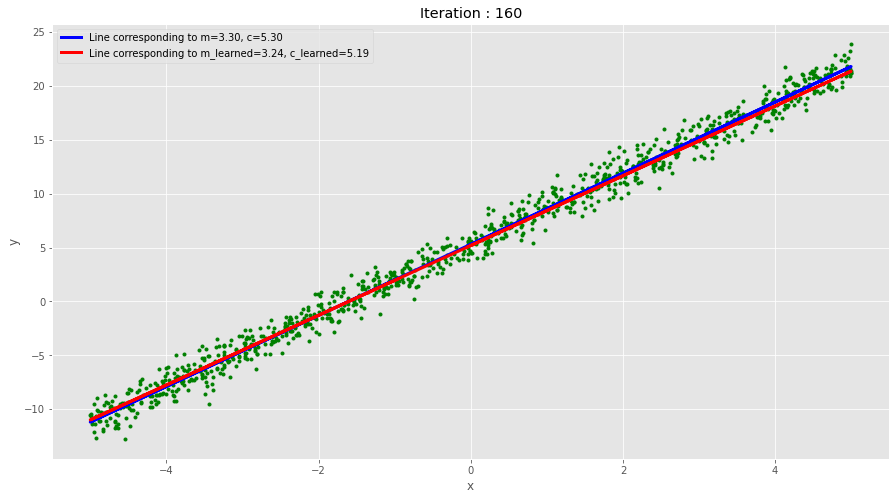
\includegraphics[width=17cm]{img/problem4_result_160.png}
	\caption{Result of gradient decent after 160 iterations}
    \label{problem4_result_160}
\end{figure}

\begin{figure}[h]
	\centering
    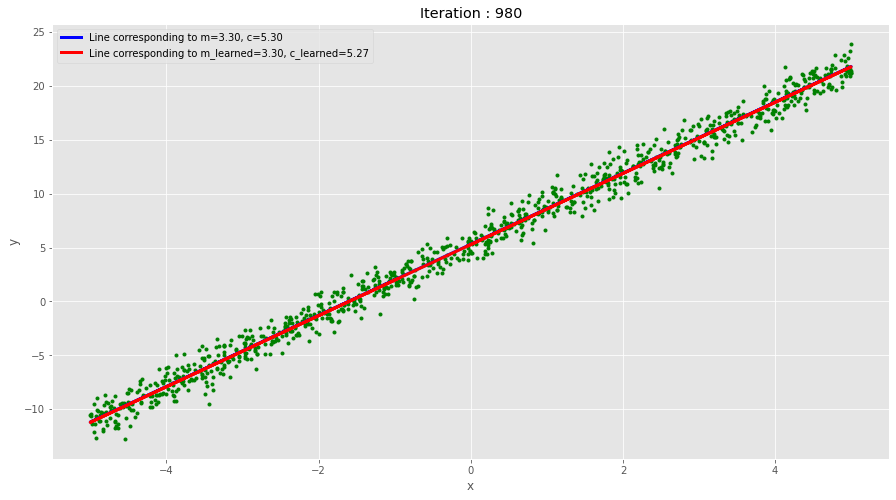
\includegraphics[width=17cm]{img/problem4_result.png}
	\caption{Result of gradient decent}
    \label{problem4_result}
\end{figure}

The loss is also plotted in figure~\ref{problem4_result_loss}.

\begin{figure}[h]
	\centering
    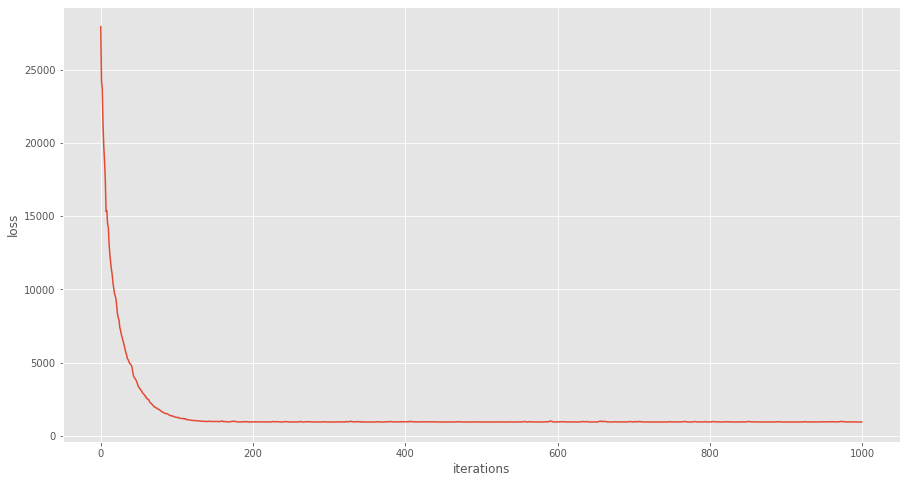
\includegraphics[width=17cm]{img/problem4_result_loss.png}
    \caption{Loss of the gradient decent over the iterations}
    \label{problem4_result_loss}
\end{figure}
